% comment out for student version
\ifdefined\Student\relax\else\def\Teacher{}\fi

\documentclass[12pt]{article}

\title{Interfaces and Abstract Classes}
\author{Nathan Sprague and Chris Mayfield}
\date{Summer 2021}

%\ProvidesPackage{cspogil}

% fonts
\usepackage[utf8]{inputenc}
\usepackage[T1]{fontenc}
\usepackage{mathpazo}

% spacing
\usepackage[margin=2cm]{geometry}
\renewcommand{\arraystretch}{1.4}
\setlength{\parindent}{0pt}

% orphans and widows
\clubpenalty=10000
\widowpenalty=10000
\pagestyle{empty}

% figures and tables
\usepackage{graphicx}
\usepackage{multicol}
\usepackage{tabularx}
\usepackage{wrapfig}

% fixed-width columns
\usepackage{array}
\newcolumntype{L}[1]{>{\raggedright\let\newline\\\arraybackslash\hspace{0pt}}m{#1}}
\newcolumntype{C}[1]{>{\centering\let\newline\\\arraybackslash\hspace{0pt}}m{#1}}
\newcolumntype{R}[1]{>{\raggedleft\let\newline\\\arraybackslash\hspace{0pt}}m{#1}}

% include paths
\makeatletter
\def\input@path{{Models/}{../../Models/}}
\graphicspath{{Models/}{../../Models/}}
\makeatother

% colors
\usepackage[svgnames,table]{xcolor}
\definecolor{bgcolor}{HTML}{FAFAFA}
\definecolor{comment}{HTML}{007C00}
\definecolor{keyword}{HTML}{0000FF}
\definecolor{strings}{HTML}{B20000}

% table headers
\newcommand{\tr}{\bf\cellcolor{Yellow!10}}

% syntax highlighting
\usepackage{textcomp}
\usepackage{listings}
\lstset{
    basicstyle=\ttfamily\color{black},
    backgroundcolor=\color{bgcolor},
    numberstyle=\scriptsize\color{comment},
    commentstyle=\color{comment},
    keywordstyle=\color{keyword},
    stringstyle=\color{strings},
    columns=fullflexible,
    keepspaces=true,
    showlines=true,
    showstringspaces=false,
    upquote=true
}

% code environments
\newcommand{\java}[1]{\lstinline[language=java]{#1}}%[
\lstnewenvironment{javalst}{\lstset{language=java,backgroundcolor=}}{}
\lstnewenvironment{javabox}{\lstset{language=java,frame=single,numbers=left}\quote}{\endquote}

% PDF properties
\usepackage[pdftex]{hyperref}
\urlstyle{same}
\makeatletter
\hypersetup{
  pdftitle={\@title},
  pdfauthor={\@author},
  pdfsubject={\@date},
  pdfkeywords={},
  bookmarksopen=false,
  colorlinks=true,
  citecolor=black,
  filecolor=black,
  linkcolor=black,
  urlcolor=blue
}
\makeatother

% titles
\makeatletter
\renewcommand{\maketitle}{\begin{center}\LARGE\@title\end{center}}
\makeatother

% boxes [optional height]
\newcommand{\emptybox}[1][10em]{
\vspace{1em}
\begin{tabularx}{\linewidth}{|X|}
\hline\\[#1]\hline
\end{tabularx}}

% models
\newcommand{\model}[1]{\section{#1}\nopagebreak}
\renewcommand{\thesection}{Model~\arabic{section}}

% questions
\newcommand{\quest}[1]{\subsection*{Questions~ (#1)}}
\newcounter{question}
\newcommand{\Q}{\vspace{1em}\refstepcounter{question}\arabic{question}.~ }
\renewcommand{\thequestion}{\#\arabic{question}}

% sub-question lists
\usepackage{enumitem}
\setenumerate[1]{label=\alph*)}
\setlist{itemsep=1em,after=\vspace{1ex}}

% inline answers
\definecolor{answers}{HTML}{C0C0C0}
\newcommand{\ans}[1]{%
\ifdefined\Student
    \leavevmode\phantom{~~\textcolor{answers}{#1}}
\else
    ~~\textcolor{answers}{#1}
\fi}

% longer answers [optional height]
\newsavebox{\ansbox}
\newenvironment{answer}[1][4em]{
\nopagebreak
\begin{lrbox}{\ansbox}
\begin{minipage}[t][#1]{\linewidth}
\color{answers}
}{
\end{minipage}
\end{lrbox}
\ifdefined\Student
    \phantom{\usebox{\ansbox}}%
\else
    \usebox{\ansbox}%
\fi}


\begin{document}

\maketitle

\begin{center}
\vspace{-1em}
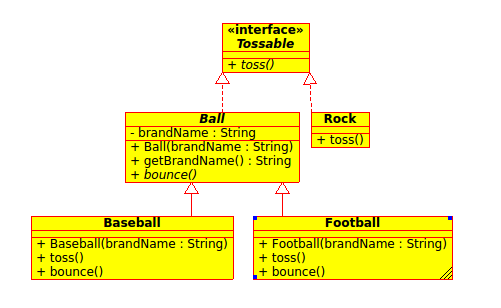
\includegraphics[scale=0.80]{interface-uml.png}
\vspace{-2em}
\end{center}


\Q Fill in each cell of the table with one of three values:

\begin{itemize}[itemsep=2pt]
\item ~\textbf{Y}~
An object of this type could be assigned to a variable of this type.
\item ~\textbf{N}~
An object of this type could \textit{not} be assigned to a variable of this type.
\item ~\textbf{--} ~
It is not possible to instantiate an object of this type.
\end{itemize}

\setlength{\defaultwidth}{3em}

\begin{center}
\begin{tabular}{|l|l|l|l|l|l|l|} \hline
\multicolumn{2}{|l|}{\multirow{2}{*}{}}   & \multicolumn{5}{c|}{\bf Variable Type}
  \\ \cline{3-7} \multicolumn{2}{|l|}{}
           & Tossable & Ball     & Rock     & Baseball & Football \\ \hline
\multirow{5}{*}{\bf Object Type}
& Tossable & \ans{--} & \ans{--} & \ans{--} & \ans{--} & \ans{--} \\ \cline{2-7} 
& Ball     & \ans{--} & \ans{--} & \ans{--} & \ans{--} & \ans{--} \\ \cline{2-7} 
& Rock     & \ans{Y}  & \ans{N}  & \ans{Y}  & \ans{N}  & \ans{N}  \\ \cline{2-7} 
& Baseball & \ans{Y}  & \ans{Y}  & \ans{N}  & \ans{Y}  & \ans{N}  \\ \cline{2-7} 
& Football & \ans{Y}  & \ans{Y}  & \ans{N}  & \ans{N}  & \ans{Y}  \\ \hline
\end{tabular}
\end{center}


\Q Write the source code for the UML diagram.

\begin{itemize}

\item In \textit{Rock.java}, the \java{toss} method should print \java{"Tossing a Rock!"}.

\item In \textit{Baseball.java}, the \java{toss} method should print \java{"Tossing a Baseball!"}, and the \java{bounce} method should print \java{"Bouncing a Baseball!"}.

\item In \textit{Football.java}, the \java{toss} method should print \java{"Tossing a Football!"}, and the \java{bounce} method should print \java{"Bouncing a Football!"}.

\end{itemize}


\Q Indicate whether each code snippet will:

\begin{itemize}[itemsep=1ex]
\item \textbf{N} ~--~ not compile;
\item \textbf{X} ~--~ compile but generate an exception at run-time; or
\item \textbf{R} ~--~ compile and run without generating an exception.
\end{itemize}


\begin{center}
\begin{tabular}{|l|l|l|} \hline
& \bf Code Snippet
& \bf Result
\\ \hline

a) &
\begin{javalst}
Ball ball = new Football("Spalding");
\end{javalst}
& \ans{R}
\\ \hline

b) &
\begin{javalst}
Ball ball = new Football("Spalding");
Baseball baseball = (Baseball) ball;
\end{javalst}
& \ans{X}
\\ \hline

c) &
\begin{javalst}
Object obj = new Baseball("Spalding");
\end{javalst}
& \ans{R}
\\ \hline

d) &
\begin{javalst}
Object obj = new Baseball("Spalding");
Tossable tossable = obj;
\end{javalst}
& \ans{N}
\\ \hline

e) &
\begin{javalst}
Tossable tossable = new Baseball("Spalding");
Object obj = tossable;
\end{javalst}
& \ans{R}
\\ \hline

f) &
\begin{javalst}
Tossable tossable = new Baseball("Spalding");
tossable.getBrandName();
\end{javalst}
& \ans{N}
\\ \hline

\end{tabular}
\end{center}


\end{document}
